\documentclass{beamer}
\mode<presentation> {
    \usetheme{CambridgeUS}
    \usecolortheme{dolphin}
}
\setbeamercolor*{title}{use=structure,fg=white,bg=structure.fg}

\setbeamertemplate{section in toc}{\color{structure}\inserttocsectionnumber.\color{black}~\inserttocsection\par}
\setbeamertemplate{subsection in toc}{\color{structure}~~\inserttocsectionnumber.\inserttocsubsectionnumber.\color{black}~\inserttocsubsection\par}
\setbeamertemplate{itemize items}[default]
\setbeamertemplate{enumerate items}[default]

\setbeamertemplate{bibliography entry title}{}
\setbeamertemplate{bibliography entry location}{}
\setbeamertemplate{bibliography entry note}{}

\usepackage[latin1]{inputenc}
\usepackage{lmodern}
\usepackage{graphicx}
\usepackage{eurosym}
\usepackage{media9}
\usepackage{tikz}

%----------------------------------------------------------------------------------------------------------------------

\title[Robots in Education]{Robots and Programming in Education}
\author{\^Angela Cardoso}
\institute[MIEIC - FEUP]{Master in Informatics and Computing Engineering \\
    \smallskip
    Faculty of Engineering of the University of Porto \\
}

\date{\today} 

\begin{document}

%----------------------------------------------------------------------------------------------------------------------

%%%%%%%%%%%%%%
% TITLE PAGE %
%%%%%%%%%%%%%%
\begin{frame}
\titlepage
\end{frame}

%----------------------------------------------------------------------------------------------------------------------

%%%%%%%%%%%%
% OVERVIEW %
%%%%%%%%%%%%
\begin{frame}
\frametitle{Overview} 
\small
\tableofcontents
\end{frame}

%----------------------------------------------------------------------------------------------------------------------

%%%%%%%%
% STEM %
%%%%%%%%
\section{Introduction} 
\subsection{STEM Education} 
\begin{frame}
\frametitle{STEM Education}
\huge{\color{structure}{S}}\visible<2->{cience}\\
\huge{\color{structure}{T}}\visible<3->{echnology}\\
\huge{\color{structure}{E}}\visible<4->{ngineering}\\
\only<6-7>{\huge{\color{structure}{A}}}\only<7>{rt}\only<6-7>{\\}
\huge{\color{structure}{M}}\visible<5->{athematics}\\
\only<8->{\huge{\color{structure}{+}}\\}
\only<8->{\huge{\color{structure}{C}}}\only<9>{omputing}\only<10>{oding}\only<11>{omputer Science}\only<8->{\\}
\end{frame}

%----------------------------------------------------------------------------------------------------------------------

%%%%%%%%%%%%%%%
% MATHEMATICS %
%%%%%%%%%%%%%%%
\subsection{Robots in STEM Education} 
\begin{frame}
\frametitle{Mathematics}
\setbeamercovered{transparent}
\begin{itemize}[<+>]
    \item Geometric primitives
    \item Counting
    \item Multiplication
    \item Decimals
    \item Fractions and ratios
    \item Coordinate systems
    \item Graphs
    \item Angles
\end{itemize}
\end{frame}

%----------------------------------------------------------------------------------------------------------------------

%%%%%%%%%%%
% PHYSICS %
%%%%%%%%%%%
\begin{frame}
\frametitle{Physics}
\setbeamercovered{transparent}
\begin{itemize}[<+>]
    \item Distance
    \item Time
    \item Velocity
    \item Acceleration
    \item Work and energy
    \item Gravity
    \item Friction
    \item Electricity
\end{itemize}
\end{frame}

%----------------------------------------------------------------------------------------------------------------------

%%%%%%%%%%%
% SCRATCH %
%%%%%%%%%%%
\section{Educational Programming Languages} 
\subsection{Scratch}
\begin{frame}
\frametitle{Scratch}
\vspace{-0.5cm}
\begin{center}
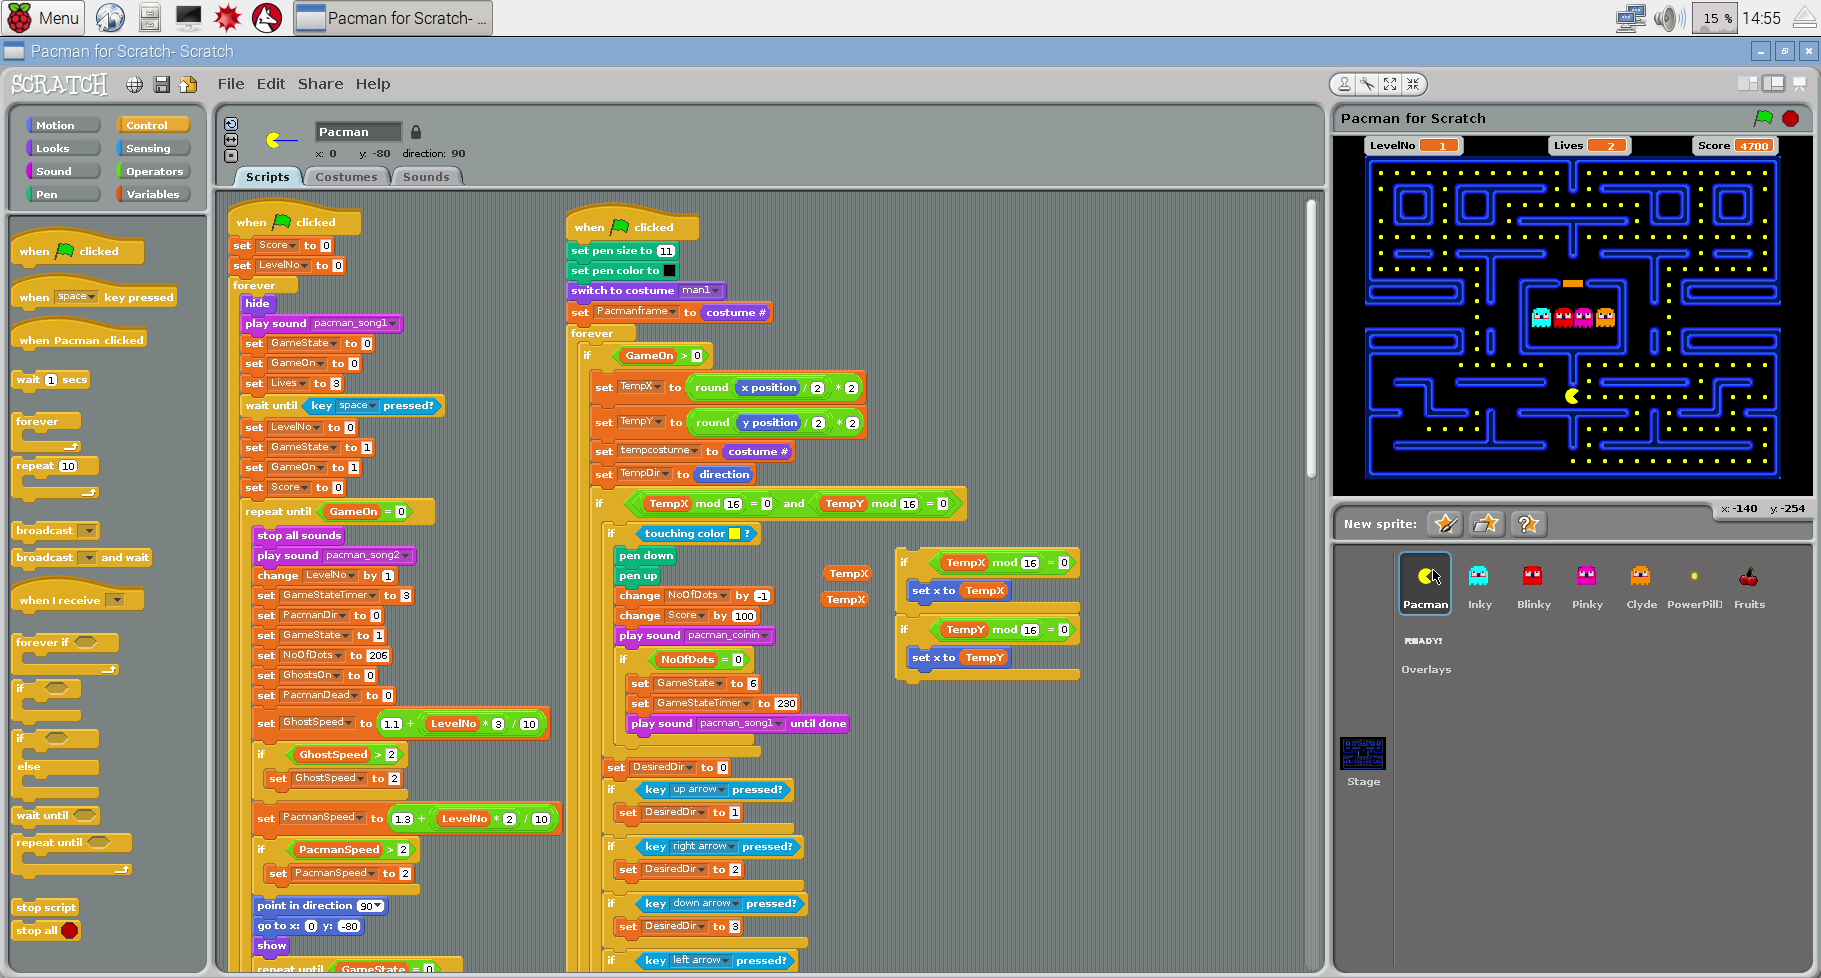
\includegraphics[scale=0.19]{images/scratch.png}
\end{center}
\end{frame}

%----------------------------------------------------------------------------------------------------------------------

%%%%%%%%%%%
% BLOCKLY %
%%%%%%%%%%%
\subsection{Blockly}
\begin{frame}
\frametitle{Blockly}
\begin{center}
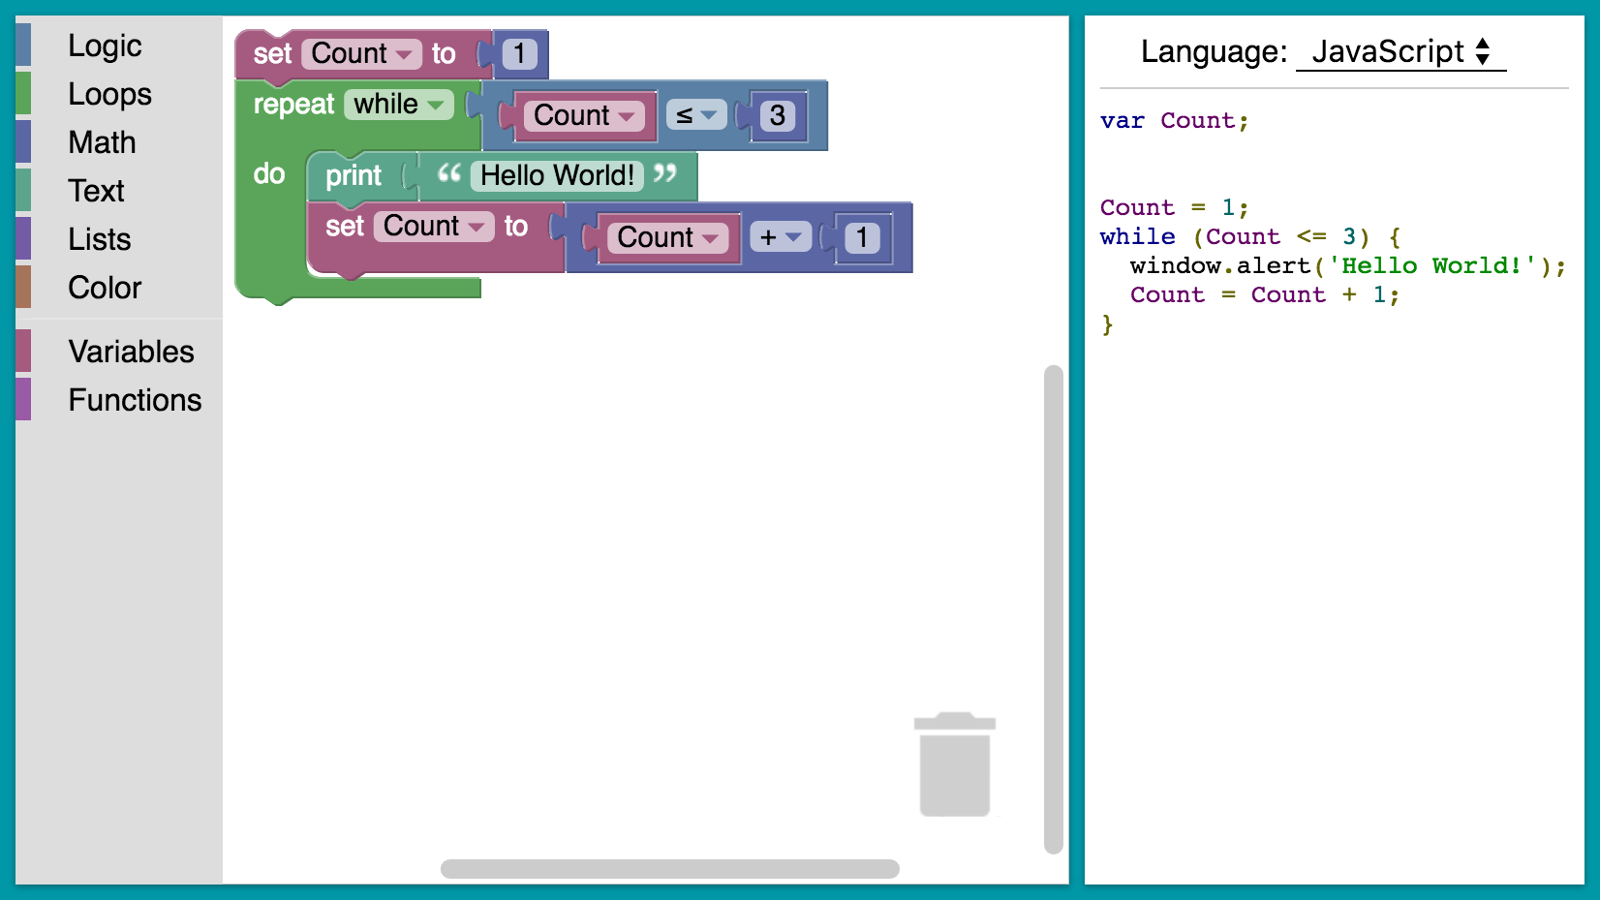
\includegraphics[scale=0.21]{images/blockly.png}
\end{center}
\end{frame}

%----------------------------------------------------------------------------------------------------------------------

%%%%%%%%%
% SWIFT %
%%%%%%%%%
\subsection{Swift Playgrounds}
\begin{frame}
\frametitle{Swift Playgrounds}
\vspace{-0.4cm}
\begin{center}
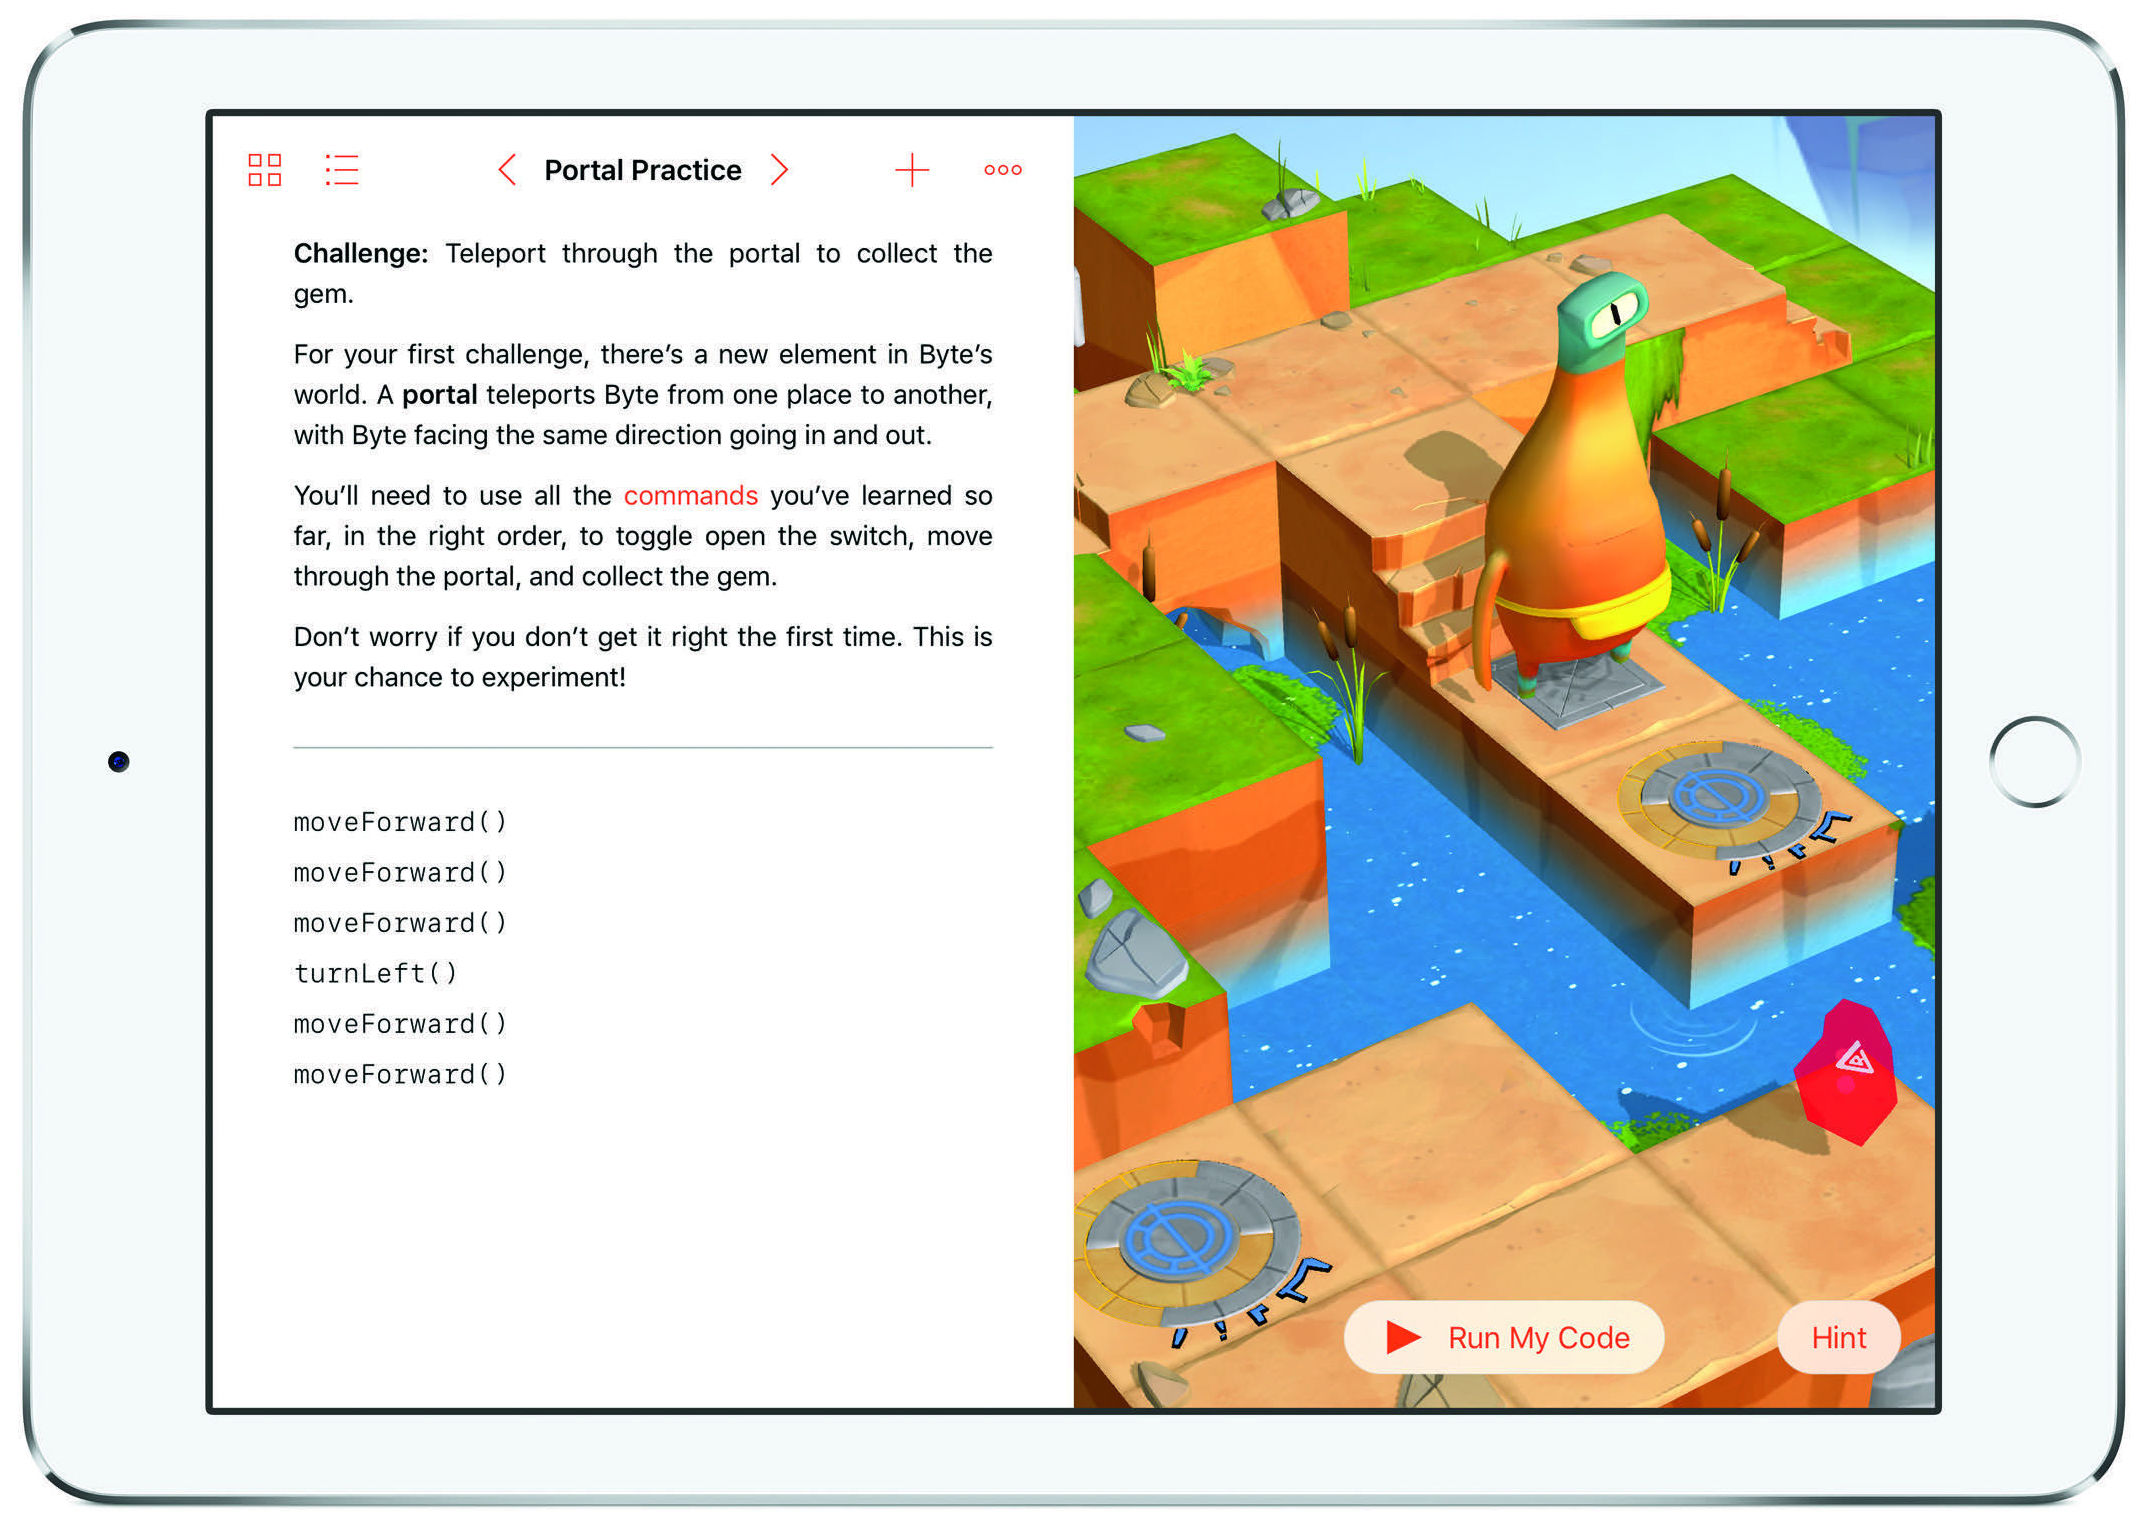
\includegraphics[scale=0.14]{images/swift.jpg}
\end{center}
\end{frame}

%----------------------------------------------------------------------------------------------------------------------

%%%%%%%%%%%%%%%%%%%%%%%
% LEGO MINDSTORMS EV3 %
%%%%%%%%%%%%%%%%%%%%%%%
\subsection{LEGO Mindstorms EV3}
\begin{frame}
\frametitle{LEGO Mindstorms EV3}
\begin{center}
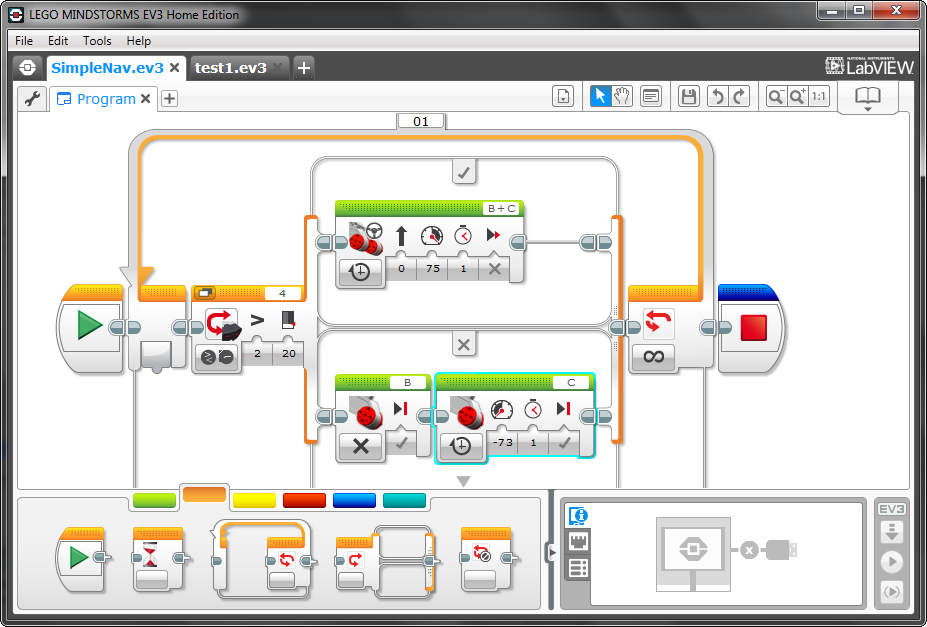
\includegraphics[scale=0.43]{images/lego.png}
\end{center}
\end{frame}

%----------------------------------------------------------------------------------------------------------------------

%%%%%%%%
% KUBO %
%%%%%%%%
\section{Educational Robots} 
\subsection{KUBO}
\begin{frame}
\frametitle{KUBO}
\begin{tikzpicture}[remember picture,overlay]
	\node[anchor=south west, inner sep=0pt] at (current page.south west) {
		\includemedia[
			addresource=videos/kubo.mp4,
            activate=pageopen,
            transparent,
            flashvars={source=videos/kubo.mp4},
            width=\paperwidth,
            height=\paperheight
  		]{}{VPlayer.swf}%
    };
\end{tikzpicture}
\end{frame}

%----------------------------------------------------------------------------------------------------------------------

%%%%%%%%%%
% THYMIO %
%%%%%%%%%%
\subsection{Thymio}
\begin{frame}
\frametitle{Thymio}
\begin{tikzpicture}[remember picture,overlay]
	\node[anchor=south west, inner sep=0pt] at (current page.south west) {
		\includemedia[
			addresource=videos/thymio.mp4,
            activate=pageopen,
            transparent,
            flashvars={source=videos/thymio.mp4},
            width=\paperwidth,
            height=\paperheight
  		]{}{VPlayer.swf}%
    };
\end{tikzpicture}
\end{frame}

%----------------------------------------------------------------------------------------------------------------------

%%%%%%%%%%%%
% CUBELETS %
%%%%%%%%%%%%
\subsection{Cubelets}
\begin{frame}
\frametitle{Cubelets}
\begin{tikzpicture}[remember picture,overlay]
	\node[anchor=south west, inner sep=0pt] at (current page.south west) {
		\includemedia[
			addresource=videos/cubelets.mp4,
            activate=pageopen,
            transparent,
            flashvars={source=videos/cubelets.mp4},
            width=\paperwidth,
            height=\paperheight
  		]{}{VPlayer.swf}%
    };
\end{tikzpicture}
\end{frame}

%----------------------------------------------------------------------------------------------------------------------

%%%%%%%%%%
% OZOBOT %
%%%%%%%%%%
\subsection{Ozobot Evo}
\begin{frame}
\frametitle{Ozobot Evo}
\begin{tikzpicture}[remember picture,overlay]
	\node[anchor=south west, inner sep=0pt] at (current page.south west) {
		\includemedia[
			addresource=videos/ozobot.mp4,
            activate=pageopen,
            transparent,
            flashvars={source=videos/ozobot.mp4},
            width=\paperwidth,
            height=\paperheight
  		]{}{VPlayer.swf}%
    };
\end{tikzpicture}
\end{frame}

%----------------------------------------------------------------------------------------------------------------------

%%%%%%%%%
% COZMO %
%%%%%%%%%
\subsection{Cozmo}
\begin{frame}
\frametitle{Cozmo}
\begin{tikzpicture}[remember picture,overlay]
	\node[anchor=south west, inner sep=0pt] at (current page.south west) {
		\includemedia[
			addresource=videos/cozmo.mp4,
            activate=pageopen,
            transparent,
            flashvars={source=videos/cozmo.mp4},
            width=\paperwidth,
            height=\paperheight
  		]{}{VPlayer.swf}%
    };
\end{tikzpicture}
\end{frame}

%----------------------------------------------------------------------------------------------------------------------

%%%%%%%%%%%%%%%%%%%
% LEGO MINDSTORMS %
%%%%%%%%%%%%%%%%%%%
\subsection{LEGO Mindstorms EV3}
\begin{frame}
\frametitle{LEGO Mindstorms EV3}
\begin{tikzpicture}[remember picture,overlay]
	\node[anchor=south west, inner sep=0pt] at (current page.south west) {
		\includemedia[
			addresource=videos/ev3.mp4,
            activate=pageopen,
            transparent,
            flashvars={source=videos/ev3.mp4},
            width=\paperwidth,
            height=\paperheight
  		]{}{VPlayer.swf}%
    };
\end{tikzpicture}
\end{frame}

%----------------------------------------------------------------------------------------------------------------------

%%%%%%%%%%%%%%
% COMPARISON %
%%%%%%%%%%%%%%
\subsection{Comparison}
\begin{frame}
\frametitle{Comparison}
\resizebox{\textwidth}{!}{
\begin{tabular}{|l|l|l|l|l|l|l|l|l|l|l|l|}
\hline
Robot     & \begin{tabular}[c]{@{}c@{}}KIBO \\ 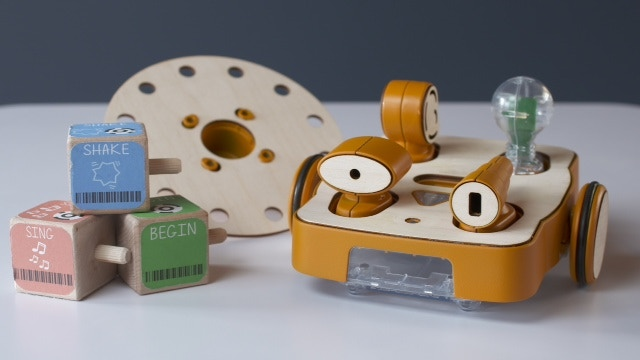
\includegraphics[scale=0.1]{images/kibo.jpg} \end{tabular} & \begin{tabular}[c]{@{}c@{}}KUBO \\ 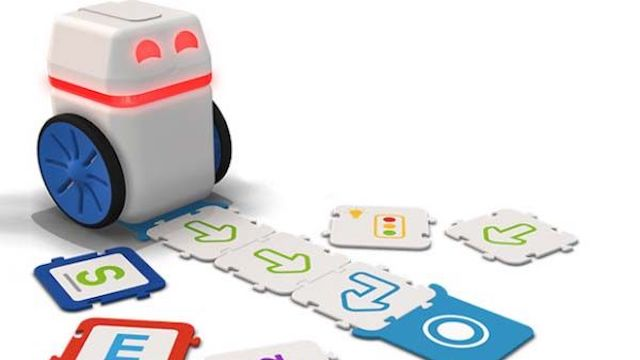
\includegraphics[scale=0.1]{images/kubo.jpg} \end{tabular} & \begin{tabular}[c]{@{}c@{}}Dash \\ 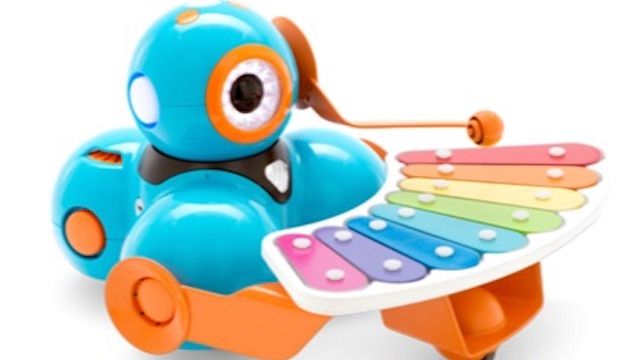
\includegraphics[scale=0.1]{images/dash.jpg} \end{tabular}        & \begin{tabular}[c]{@{}c@{}}Thymio \\ 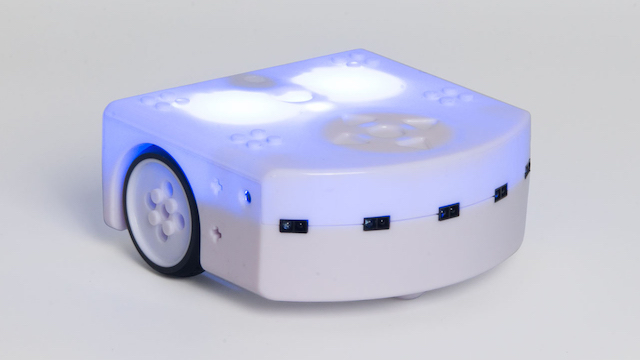
\includegraphics[scale=0.1]{images/thymio.jpg} \end{tabular}                                             & \begin{tabular}[c]{@{}c@{}}LEGO Boost \\ 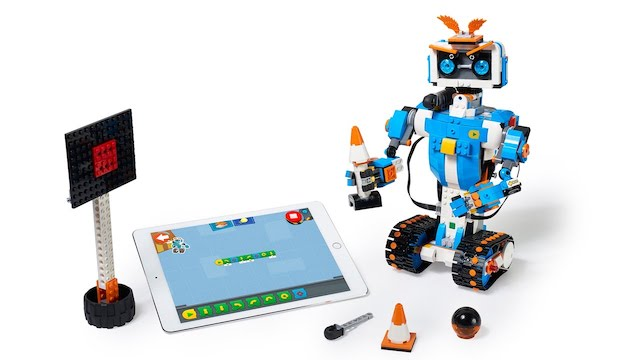
\includegraphics[scale=0.1]{images/boost.jpg} \end{tabular} & \begin{tabular}[c]{@{}c@{}}Cubelets \\ 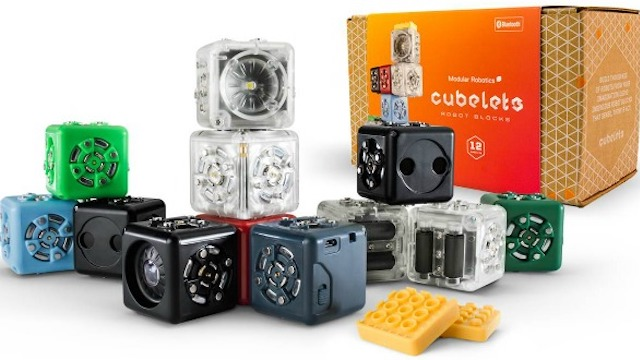
\includegraphics[scale=0.1]{images/cubelets.jpg}\end{tabular}                                       & \begin{tabular}[c]{@{}c@{}}Ozobot Evo \\ 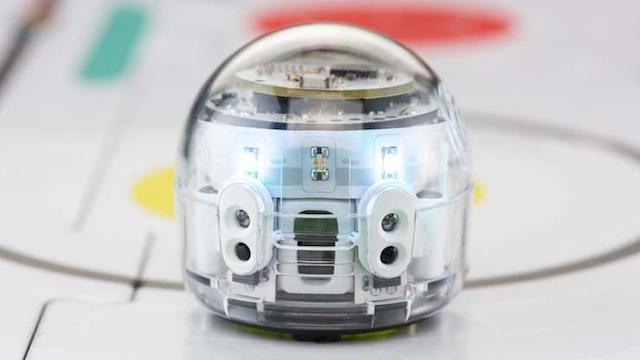
\includegraphics[scale=0.1]{images/ozobot.jpg} \end{tabular} & \begin{tabular}[c]{@{}c@{}}Sphero \\ 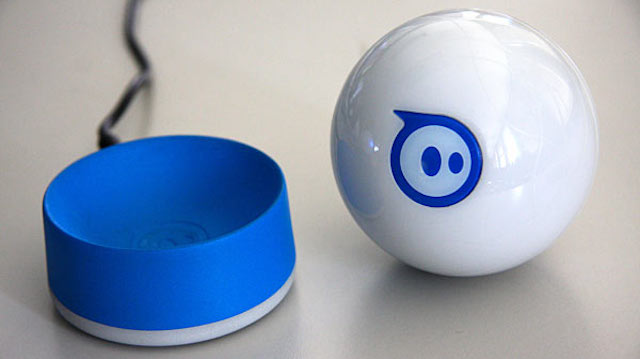
\includegraphics[scale=0.1]{images/sphero.jpg} \end{tabular}                & \begin{tabular}[c]{@{}c@{}}Cozmo \\ 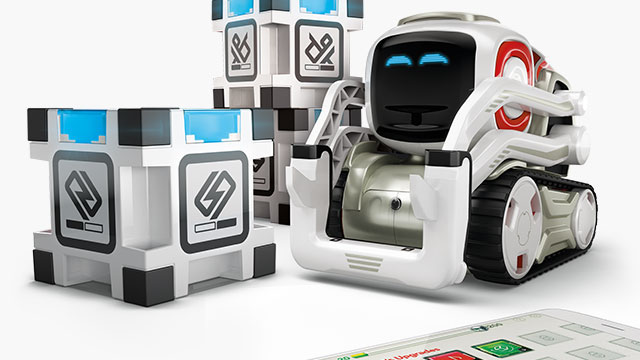
\includegraphics[scale=0.1]{images/cozmo.jpg} \end{tabular} & \begin{tabular}[c]{@{}c@{}}LEGO EV3 \\ 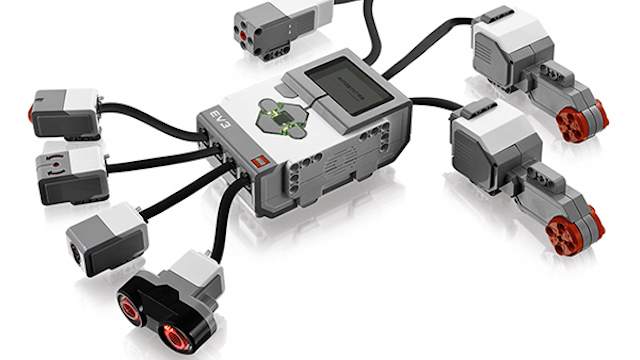
\includegraphics[scale=0.1]{images/ev3.jpg}\end{tabular}         & \begin{tabular}[c]{@{}c@{}}Parrot Jumping \\ 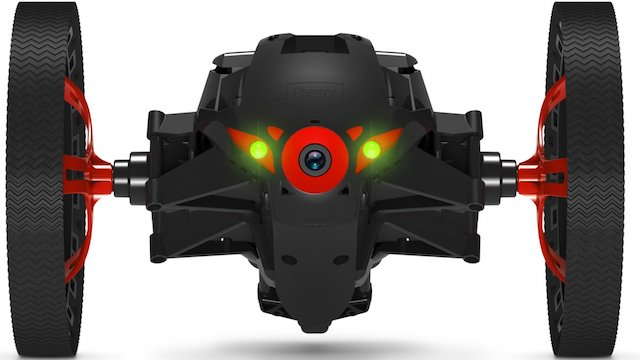
\includegraphics[scale=0.1]{images/parrot.jpg} \end{tabular}   \\ \hline
Price     & \EUR{195} - \EUR{425}                                                             	   		  & \EUR{370}                                                                   	  			  & \EUR{130}                                                                                            & \EUR{130}                                                                                                                                     & \EUR{160}                                                                                 			& \EUR{135} - \EUR{425}                                                                                                                      & \EUR{85}                                                                                 			 & \EUR{110}                                                                                                        & \EUR{165}                                                                                       & \EUR{400}                                                                                               & \EUR{80}                                                                     	   								  \\ \hline
Age       & 4 - 7                                                                 	   		 			  & 4 - 10                                                                	  					  & 5 - 8                                                                                                & 6+                                                                                                                                            & 7 - 10                                                                             					& 8+                                                                                                                                     	 & 8+                                                                                 					 & 8+                                                                                                               & 8+                                                                                              & 10+                                                                                                     & 10+                                                                    	   								  \\ \hline
Coding    & Wood Blocks                                                                		 			  & TagTile                                                               	  					  & \begin{tabular}[c]{@{}l@{}}Blockly\\ Swift Playgrounds\end{tabular}                                  & \begin{tabular}[c]{@{}l@{}}VPL\\ Blockly\\ Scratch\end{tabular}                                                                               & Boost                                                                               					& \begin{tabular}[c]{@{}l@{}}Cubelets\\ Blockly\end{tabular}                                                                             	 & \begin{tabular}[c]{@{}l@{}}OzoCodes\\ Blockly\end{tabular}                         					 & \begin{tabular}[c]{@{}l@{}}Sphero Macrolab\\ orbBasic\end{tabular}                                               & \begin{tabular}[c]{@{}l@{}}Code Lab\\ Python\end{tabular}                                       & \begin{tabular}[c]{@{}l@{}}LEGO EV3\\ LabVIEW\\ RoboC\\ Scratch\end{tabular}                            & Scratch                                                                	   								  \\ \hline
Bulding   & yes                                                                   	   		 			  & no                                                                    	  					  & some                                                                                                 & no                                                                                                                                            & multiple                                                                            					& yes                                                                                                                                    	 & no                                                                                 					 & no                                                                                                               & no  	                                                                                          & multiple                                                                                                & no                                                                     	   								  \\ \hline
Sensors   & \begin{tabular}[c]{@{}l@{}}sound\\ light\\ distance\end{tabular}      	   		 			  & tile recog.                                                      	   	  					  & \begin{tabular}[c]{@{}l@{}}3 microphones\\ 3 distance\end{tabular}                                   & \begin{tabular}[c]{@{}l@{}}9 IR proximity\\ 5 cap. touch but.\\ 1 accelerometer\\ 1 thermometer\\ 1 microphone\end{tabular} 					 & \begin{tabular}[c]{@{}l@{}}color\\ distance\end{tabular}                            					& \begin{tabular}[c]{@{}l@{}}1 brightness\\ 2 distance\\ 1 temperature\\ 1 knob\end{tabular}                                             	 & \begin{tabular}[c]{@{}l@{}}IR proximity\\ optical\end{tabular}                     					 & \begin{tabular}[c]{@{}l@{}}accelerometer\\ gyroscope\end{tabular}                                                & \begin{tabular}[c]{@{}l@{}}vga camera\\ gyroscope \\ accelerometer \end{tabular}                & \begin{tabular}[c]{@{}l@{}}1 color\\ 2 touch\\ 1 ultrasonic\\ 1 gyro\end{tabular}                       & \begin{tabular}[c]{@{}l@{}}accelerometer\\ gyroscope\end{tabular}      	   								  \\ \hline
Actuators & \begin{tabular}[c]{@{}l@{}}LEDs\\ wheels\end{tabular}                	   		 			  & \begin{tabular}[c]{@{}l@{}}wheels\\ LEDs\end{tabular}                  	  					  & \begin{tabular}[c]{@{}l@{}}wheels\\ 1 speaker\\ 12 white LEDs\\ 3 RGB LEDs\\ 1 red LED\end{tabular}  & \begin{tabular}[c]{@{}l@{}}39 LEDs\\ 2 DC motors\\ 1 loud-speaker\end{tabular}                                                                & \begin{tabular}[c]{@{}l@{}}move hub\\ motor\end{tabular}                            					& \begin{tabular}[c]{@{}l@{}}1 rotate\\ 2 wheels\\ 1 light\\ 1 speaker\\ 1 bar graph\end{tabular}                                        	 & \begin{tabular}[c]{@{}l@{}}LEDs\\ speaker\\ wheels\end{tabular}                    					 & \begin{tabular}[c]{@{}l@{}}LEDs\\ int. wheels\end{tabular}                                        			    & \begin{tabular}[c]{@{}l@{}}4 motors\\ OLED display \\ speaker\end{tabular}                      & \begin{tabular}[c]{@{}l@{}}2 large motors\\ 1 small motor\\ 1 display\\ 1 speaker\\ lights\end{tabular} & \begin{tabular}[c]{@{}l@{}}wheels\\ jumping\end{tabular}               	   								  \\ \hline
Other     &                                                                       	   		 			  &                                                                       	  					  & \begin{tabular}[c]{@{}l@{}}2 IR receivers\\ 3 IR transmitters\\ xylophone\\ accessories\end{tabular} & \begin{tabular}[c]{@{}l@{}}hold pencil\\ follows lines\\ pull trailer\\ microSD card\\ 6 behaviours\\ 1 IR receiver\\ 1 wireless\end{tabular} &                                                                                     					& \begin{tabular}[c]{@{}l@{}}1 bluetooth\\ 2 block\\ 1 minimum\\ 1 maximum\\ 2 inverse\end{tabular}                                      	 & app RC                                                                			 					 & \begin{tabular}[c]{@{}l@{}}bluetooth\\ app RC\end{tabular}                                                       & \begin{tabular}[c]{@{}l@{}}facial recog.\\ app control\end{tabular}                             & \begin{tabular}[c]{@{}l@{}}IR RC\\ bluetooth\end{tabular}                                   			& \begin{tabular}[c]{@{}l@{}}VGA camera\\ app RC\end{tabular}   			   								  \\ \hline
Pros      & \begin{tabular}[c]{@{}l@{}}preschoolers\\ no screen \\~~~code\end{tabular} 		 			  & \begin{tabular}[c]{@{}l@{}}preschoolers\\ no screen\\~~code\end{tabular} 					  & \begin{tabular}[c]{@{}l@{}}cheap\\ multilanguage\\ LEGO compat.\end{tabular}                         & \begin{tabular}[c]{@{}l@{}}cheap\\ multilanguages\\ lots of sensors\\ lots of features\\ powerful\end{tabular}                                & \begin{tabular}[c]{@{}l@{}}infinite robots\\ LEGO compat.\end{tabular}              					& \begin{tabular}[c]{@{}l@{}}building is coding\\ no screen\\~~~code\\ multiple sensors\\ multiple actuators\\ different robots\end{tabular} & \begin{tabular}[c]{@{}l@{}}cheap\\ no screen code\end{tabular}                     					 & cheap                                                                                                        	& \begin{tabular}[c]{@{}l@{}}cute\\ has sdk \end{tabular}                                         & \begin{tabular}[c]{@{}l@{}}infinite robots\\ powerful\\ LEGO compat.\end{tabular}                  	    & \begin{tabular}[c]{@{}l@{}}cheap\\ has sdk \end{tabular}                                                    \\ \hline
Cons      & \begin{tabular}[c]{@{}l@{}}expensive\\ simple code\end{tabular}  	  	   		 			  & \begin{tabular}[c]{@{}l@{}}expensive\\ simple code\end{tabular}  	   	  					  & \begin{tabular}[c]{@{}l@{}}few sensors\\ needs comp.\\~~~or tablet\end{tabular}                      & \begin{tabular}[c]{@{}l@{}}needs comp.\\~~~or tablet\end{tabular}                                                                             & \begin{tabular}[c]{@{}l@{}}specific code\\ few sensors\\ few actuators\end{tabular} 					& \begin{tabular}[c]{@{}l@{}}full kit expensive\\ small kit lacking\end{tabular}                                                         	 & \begin{tabular}[c]{@{}l@{}}few sensors\\ few actuators\\ few features\end{tabular} 					 & \begin{tabular}[c]{@{}l@{}}needs phone \\~~~or tablet\\ few sensors\\ few actuators\\ specific code\end{tabular} & \begin{tabular}[c]{@{}l@{}}needs phone \\~~~or tablet\\ few sensors\\ \end{tabular} 			  & \begin{tabular}[c]{@{}l@{}}expensive\\ expensive extras\\ paid software\end{tabular}                    & \begin{tabular}[c]{@{}l@{}}needs iOS\\~~~device\\ few sensors\end{tabular} 								  \\ \hline
\end{tabular}
}
\end{frame}


%----------------------------------------------------------------------------------------------------------------------

%%%%%%%%%%%%%%
% CONCLUSION %
%%%%%%%%%%%%%%
\section{Conclusion}
\begin{frame}
\frametitle{Which Robot?}
\visible<+->{Robots can be a great educational tool. Which robot is best?}
\begin{itemize}[<+->]
	\item Want something cheap? Get Ozobot Evo! Good relation value/price, supports both no screen coding and Blockly.
	\item Want many sensors? Get Thymio! Good relation value/price, probably most feature packed robot here.
	\item Want to build at will? Get LEGO Mindstorms EV3! Bit expensive, but you may build infinite robots.
	\item Want something different? Get Cubelets! Full pack is quite expensive, but you can build and code at the same time.
\end{itemize}
\end{frame}

%----------------------------------------------------------------------------------------------------------------------

\begin{frame}
\frametitle{The trends?}
\visible<+->{STEM education, and coding in particular, are on the rise in schools. What are the trends?}
\begin{itemize}[<+->]
	\item Introduce coding to kids very early, even before they can read.
	\item Use symbols instead of text, graphical coding.
	\item Code without a screen.
	\item Affordable and easy to program robots.
	\item Robots that can grow in complexity, for example, programmable with different languages.
\end{itemize}
\end{frame}

%----------------------------------------------------------------------------------------------------------------------

%%%%%%%%%%%%%%%%
% BIBLIOGRAPHY %
%%%%%%%%%%%%%%%%
\section{Bibliography}
\begin{frame}
\frametitle{Bibliography}
	{\scriptsize
        \bibliographystyle{amsalpha}
    	\nocite{*}
    	\bibliography{SoA_presentation}
 	}
\end{frame}

\end{document} 
